% Created 2021-07-20 Tue 10:14
% Intended LaTeX compiler: pdflatex
\documentclass[presentation,aspectratio=169]{beamer}
\usepackage[utf8]{inputenc}
\usepackage[T1]{fontenc}
\usepackage{graphicx}
\usepackage{grffile}
\usepackage{longtable}
\usepackage{wrapfig}
\usepackage{rotating}
\usepackage[normalem]{ulem}
\usepackage{amsmath}
\usepackage{textcomp}
\usepackage{amssymb}
\usepackage{capt-of}
\usepackage{hyperref}
\usepackage{khpreamble}
\usepackage{amssymb}
\DeclareMathOperator{\shift}{q}
\DeclareMathOperator{\diff}{p}
\usetheme{default}
\author{Kjartan Halvorsen}
\date{\today}
\title{Polynomial pole placement - part 2}
\hypersetup{
 pdfauthor={Kjartan Halvorsen},
 pdftitle={Polynomial pole placement - part 2},
 pdfkeywords={},
 pdfsubject={},
 pdfcreator={Emacs 26.3 (Org mode 9.4.6)}, 
 pdflang={English}}
\begin{document}

\maketitle


\section{Intro}
\label{sec:org8bb9cb2}

\begin{frame}[label={sec:orgef2154c}]{Goal of today's lecture}
Understand the design procedure of polynomial pole placement
\end{frame}


\section{2-dof controller}
\label{sec:orga4e419a}

\begin{frame}[label={sec:org6dfc545}]{Two-degree-of-freedom controller}
\begin{center}
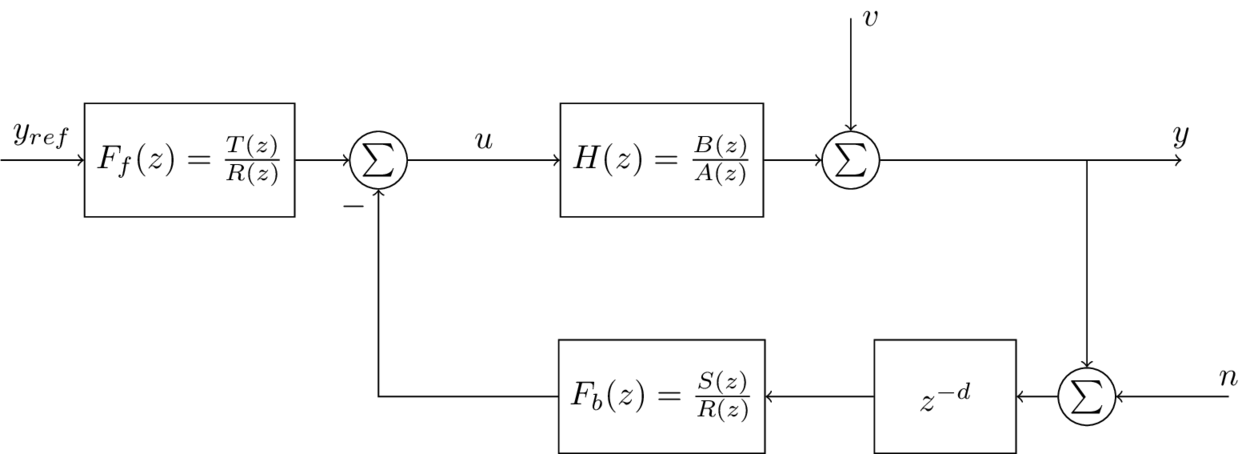
\includegraphics[width=0.7\linewidth]{../../figures/2dof-block-explicit}
\end{center}

\begin{align*}
Y(z)     &= \frac{F_f(z)H(z)}{1 + z^{-d}F_b(z)H(z)}U_c(z) + \overbrace{\frac{1}{1 + z^{-d}F_b(z)H(z)}}^{S_s(z)}V(z)  - \overbrace{\frac{z^{-d}F_b(z)H(z)}{1 + z^{-d}F_b(z)H(z)}}^{T_s(z)}N(z)\\
\end{align*}

\alert{Evidently} \(S_s(z) + T_s(z) = 1\) \alert{Conclusion:} One must find a balance between disturbance rejection and noise attenuation.
\end{frame}


\section{Sensitivity, revisited}
\label{sec:orgaa3ab2a}
\begin{frame}[label={sec:org523ac99}]{The sensitivity function}
\[S_s(z) = \frac{1}{1 + z^{-d}F_b(z)H(z)} = \frac{1}{1 + G_o(z)}= \frac{1}{G_o(z) - (-1)}\]


\begin{columns}
\begin{column}{0.45\columnwidth}
\[|S_s(\mathrm{e}^{i\omega h})| = |S_s(i\omega)| = \frac{1}{| G_o(i\omega) - (-1)|}\]

\alert{The magnitude of the sensitivity function is inverse proportional to the distance of the Nyquist curve to the critical point -1}
\end{column}

\begin{column}{0.65\columnwidth}
\begin{center}
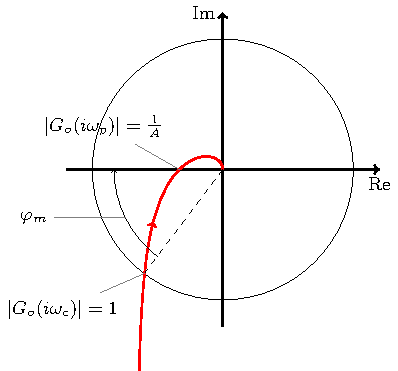
\includegraphics[width=0.6\linewidth]{../../figures/implane-nyquist-margins}
\end{center}
\end{column}
\end{columns}
\end{frame}



\section{RST}
\label{sec:orgb0db44e}

\begin{frame}[label={sec:org73a5512}]{The design procedure}
\end{frame}
\begin{frame}[label={sec:org07f51fc}]{The design procedure}
Given plant model \(H(z)=\frac{B(z)}{A(z)}\) and specifications on the desired closed-loop poles \(A_{cl}(z)\)
\begin{enumerate}
\item Find polynomials \(R(z)\) and \(S(z)\) with \(n_R \ge n_S\) such that 
\[ A(z)R(z)z^{d} + B(z)S(z) = A_{cl}(z) \]
\item Factor the closed-loop polynomials as \(A_{cl}(z) = A_c(z)A_o(z)\), where \(n_{A_o} \le n_R\). Choose
\[T(z) = t_0 A_o(z),\] where \(t_0 = \frac{A_c(1)}{B(1)}\).
\end{enumerate}

The control law is then
\[ R(q) u(k) = T(q)u_c(k) - S(q)y(k). \]
The closed-loop response to the command signal is given by
\[ A_c(q)y(k) = t_0 B(q) u_c(k). \]
\end{frame}
\begin{frame}[label={sec:org1a53433}]{Determining the order of the controller}
With Diophantine equation 
   \[ A(z)R(z)z^{d} + B(z)S(z) = A_{cl}(z) \qquad (*) \]
and feedback controller
\[F_b(z) = \frac{S(z)}{R(z)} = \frac{s_0z^n + s_1z^{n-1} + \cdots + s_n}{z^n + r_1 z^{n-1} + \cdots + r_n}\]
\alert{How should we choose the order of the controller?} Note:
\begin{itemize}
\item the controller has \(n+n+1 = 2\deg R + 1\) unknown parameters
\item the LHS of \((*)\) has degree \(\deg \big(A(z)R(z)z^d + B(z)S(z)\big) = \deg A + \deg R + d\)
\item The diophantine gives as many (nontrivial) equations as the degree of the polynomials on each side when we set the coefficients equal.

\alert{\(\Rightarrow\;\)Choose \(\deg R\) so that \(2\deg R + 1 = \deg A + \deg R + d\)}
\end{itemize}
\end{frame}


\begin{frame}[label={sec:org2ebbb1d}]{Determining the order of the controller - Exercise}
With the plant model \[H(z) = \frac{B(z)}{A(z)} = \frac{b}{z + a}\] and \(d=0\) (no delay), what is the appropriate degree of the controller 
\[F_b(z) = \frac{S(z)}{R(z)} = \frac{s_0z^n + s_1z^{n-1} + \cdots + s_n}{z^n + r_1 z^{n-1} + \cdots + r_n}\]
so that all parameters can be determined from the diophantine equation
\[ A(z)R(z) + B(z)S(z) = A_c(z)A_o(z)?\]
\begin{center}
\begin{tabular}{ll}
1. \(n = 0\) & 2. \(n = 1\)\\
3. \(n=2\) & 4. \(n=3\)\\
\end{tabular}
\end{center}
\end{frame}

\begin{frame}[label={sec:orgefa8757}]{Determining the order of the controller - Exercise - Solution}
With the plant model \[H(z) = \frac{B(z)}{A(z)} = \frac{b}{z + a}\] and \(d=0\) (no delay), what is the appropriate degree of the controller \[F_b(z) = \frac{S(z)}{R(z)} = \frac{s_0z^n + s_1z^{n-1} + \cdots + s_n}{z^n + r_1 z^{n-1} + \cdots + r_n}\]
so that all parameters can be determined from the diophantine equation
\[ A(z)R(z) + B(z)S(z) = A_c(z)A_o(z)?\]
\begin{center}
\begin{tabular}{rr}
1. \(n = 0\) & 2.\\
3. & 4.\\
\end{tabular}
\end{center}
\end{frame}


\begin{frame}[label={sec:orgcbd8cc2}]{Two-degree-of-freedom controller, the importance of the observer poles}
\begin{center}
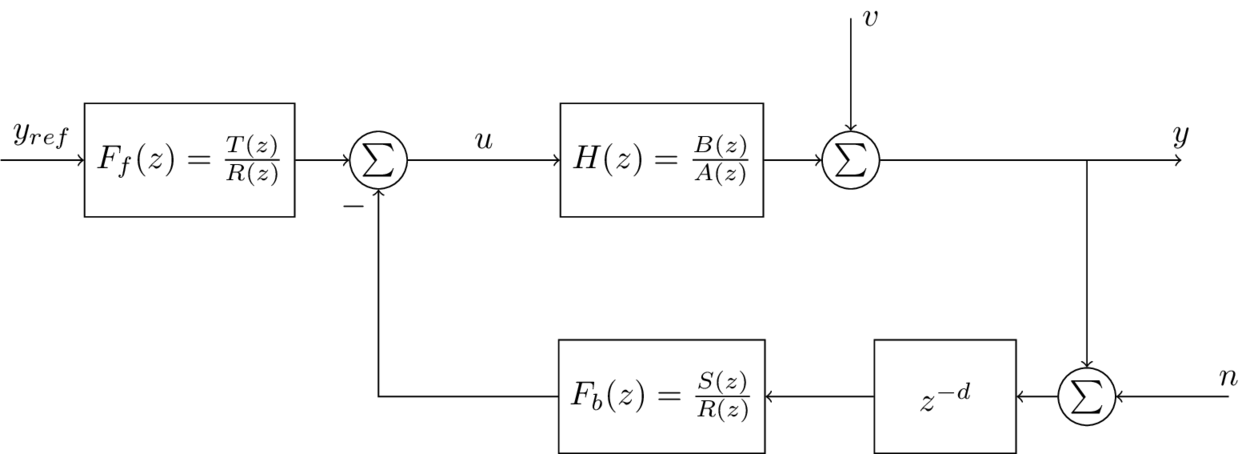
\includegraphics[width=0.7\linewidth]{../../figures/2dof-block-explicit}
\end{center}
\begin{align*}
Y(z) &= \frac{t_0B(z)z^d}{A_c(z)}U_c(z) + \frac{A(z)R(z)z^d}{A_c(z)A_o(z)}V(z)- \frac{S(z)B(z)}{A_c(z)A_o(z)}N(z)
\end{align*}
\alert{Conclusiones} 1) There is a partial separation between designing for reference tracking and designing for perturbance rejection. 2) The observer poles (the roots of \(A_o(z)\)) can be used to determine a balance between disturbance rejection and noise attenuation.
\end{frame}




\section{Example}
\label{sec:orgabd7f07}
\begin{frame}[label={sec:org2ecba8c}]{Example - Level control of a dam}
\begin{center}
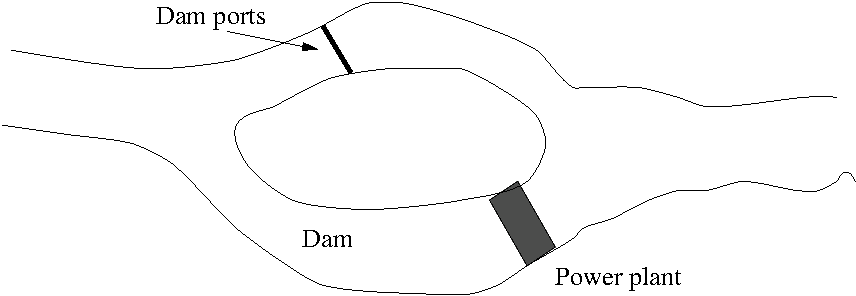
\includegraphics[width=0.5\linewidth]{../../figures/kraftverk}
\end{center}

\alert{Objective} Design a control system to maintain the water level under influence of disturbances.
\end{frame}

\begin{frame}[label={sec:org3c2cd7f}]{Example - Level control of a dam}
\begin{center}
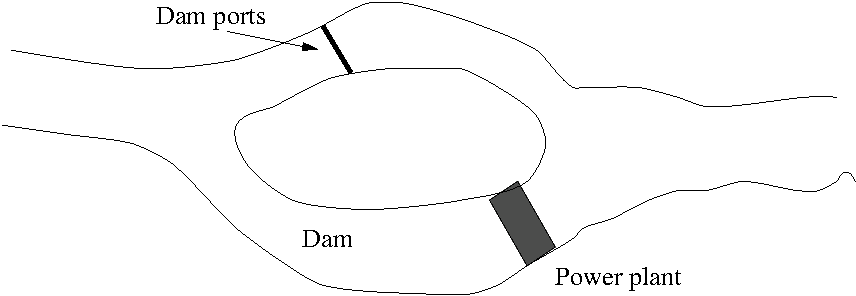
\includegraphics[width=0.3\linewidth]{../../figures/kraftverk}
\end{center}

\alert{The process dynamics}

\begin{center}
  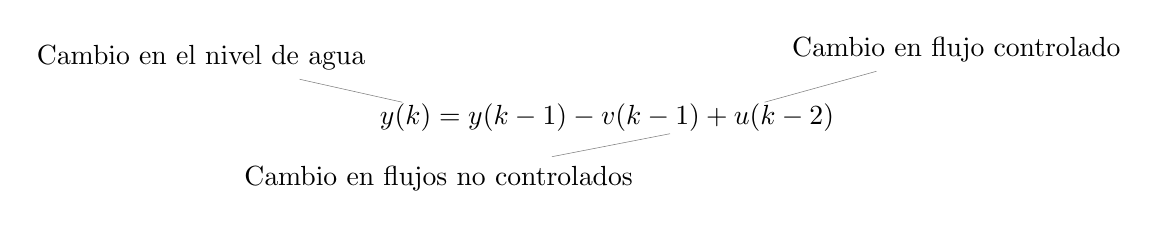
\begin{tikzpicture}
    \node at (0,0) {$y(k) = y(k-1) -v(k-1) + u(k-2)$};
    \node[coordinate, pin=140:{Cambio en el nivel de agua}] at (-2.6,0.2) {};
    \node[coordinate, pin=-140:{Cambio en flujos no controlados}] at (0.8,-0.2) {};
    \node[coordinate, pin=60:{Cambio en flujo controlado}] at (2,0.2) {};
\end{tikzpicture}
\end{center}
\begin{center}
  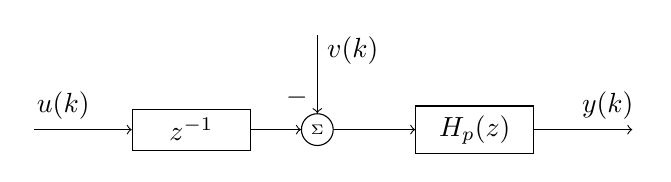
\begin{tikzpicture}[node distance=22mm, block/.style={rectangle, draw, minimum width=15mm}, sumnode/.style={circle, draw, inner sep=2pt}]

    \node[coordinate] (input) {};
    \node[block, right of=input, node distance=20mm] (delay)  {$z^{-1}$};
    \node[sumnode, right of=delay, node distance=16mm] (sum) {\tiny $\Sigma$};
    \node[block, right of=sum, node distance=20mm] (plant)  {$H_p(z)$};
    \node[coordinate, above of=sum, node distance=12mm] (disturbance) {};
    \node[coordinate, right of=plant, node distance=20mm] (output) {};

    \draw[->] (input) -- node[above, pos=0.3] {$u(k)$} (delay);
    \draw[->] (sum) -- node[above] {} (plant);
    \draw[->] (plant) -- node[above, near end] {$y(k)$} (output);
    \draw[->] (disturbance) -- node[right, pos=0.2] {$v(k)$} node[left, pos=0.8] {$-$} (sum);
    \draw[->] (delay) -- (sum);
  \end{tikzpicture}
\end{center}
\end{frame}

\begin{frame}[label={sec:org61013f5}]{Example - Level control of a dam}
\alert{The process dynamics}

\begin{center}
  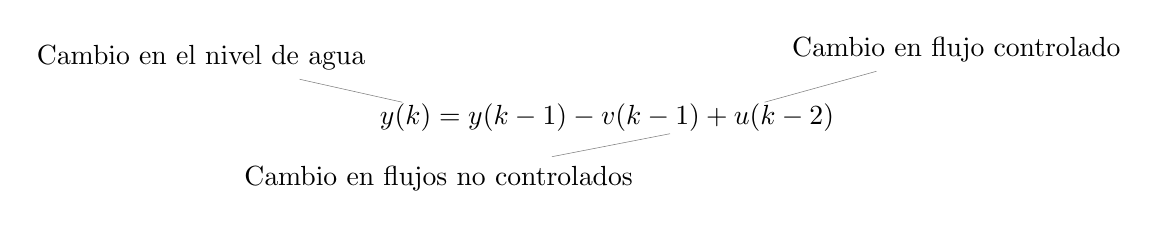
\begin{tikzpicture}
    \node at (0,0) {$y(k) = y(k-1) -v(k-1) + u(k-2)$};
    \node[coordinate, pin=140:{Cambio en el nivel de agua}] at (-2.6,0.2) {};
    \node[coordinate, pin=-140:{Cambio en flujos no controlados}] at (0.8,-0.2) {};
    \node[coordinate, pin=60:{Cambio en flujo controlado}] at (2,0.2) {};
\end{tikzpicture}
\end{center}
\begin{center}
  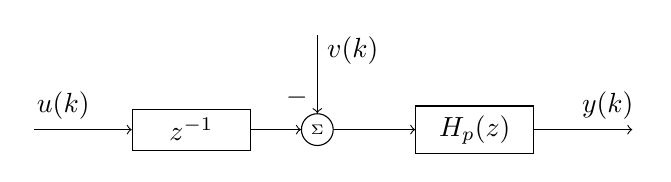
\begin{tikzpicture}[node distance=22mm, block/.style={rectangle, draw, minimum width=15mm}, sumnode/.style={circle, draw, inner sep=2pt}]

    \node[coordinate] (input) {};
    \node[block, right of=input, node distance=20mm] (delay)  {$z^{-1}$};
    \node[sumnode, right of=delay, node distance=16mm] (sum) {\tiny $\Sigma$};
    \node[block, right of=sum, node distance=20mm] (plant)  {$H_p(z)$};
    \node[coordinate, above of=sum, node distance=12mm] (disturbance) {};
    \node[coordinate, right of=plant, node distance=20mm] (output) {};

    \draw[->] (input) -- node[above, pos=0.3] {$u(k)$} (delay);
    \draw[->] (sum) -- node[above] {} (plant);
    \draw[->] (plant) -- node[above, near end] {$y(k)$} (output);
    \draw[->] (disturbance) -- node[right, pos=0.2] {$v(k)$} node[left, pos=0.8] {$-$} (sum);
    \draw[->] (delay) -- (sum);
  \end{tikzpicture}
\end{center}
\alert{Activity} What is the transfer function from \(u(k)\) to \(y(k)\)?

\begin{center}
\begin{tabular}{lll}
1: \(H(z) = \frac{z}{z-1}\) & 2: \(H(z)=\frac{1}{z-1}\) & 3: \(H(z)=\frac{1}{z(z-1)}\)\\
\end{tabular}
\end{center}
\end{frame}


\begin{frame}[label={sec:orgd0cf498}]{Example - Level control of a dam}
Given process \(H(z) = \frac{B(z)}{A(z)} = \frac{1}{z(z-1)}\) and desired poles in \(z=0.9\).

\begin{enumerate}
\item The Diophantine equation \(A(z)R(z)z^d + B(z)S(z) = A_{cl}(z)\)
\[ z(z-1)R(z) + S(z) = A_{cl}(z)\]
The order of the controller is
\[\deg R = \deg A + d - 1 = 2-1 = 1, \quad \Rightarrow \quad F_b(z)=\frac{S(z)}{R(z)} = \frac{s_0z + s_1}{z + r_1}\]
\item Resulting Diophantine equation
\[ z(z-1)(z+r_1) + s_0z + s_1 = A_{cl}(z)\]
The degree of \(A_{cl}(z)\) is 3. Choose \(A_o(z) = z\),  ( \(\deg A_o = \deg R\)) 
\[ A_{cl}(z) = A_o(z) A_c(z) = z(z-0.9)^2\]
\end{enumerate}
\end{frame}

\begin{frame}[label={sec:orgc75df91}]{Example - Level control of a dam}
\begin{enumerate}
\setcounter{enumi}{2}
\item From the Diophantine equation \[ z(z-1)(z+r_1) + s_0z + s_1 = z(z-0.9)^2\]
\[ z^3 + (r_1-1)z^2 - r_1z + s_0z + s_1 = z^3 -1.8z^2 + 0.81z\]
we obtain the equations
\begin{align*}
\begin{cases} z^2 &: \quad r_1-1 = -1.8\\
z^1 &: \quad -r_1 + s_0 = 0.81\\
z^0 &: \quad s_1 = 0
\end{cases}
\quad \Rightarrow \quad 
\begin{cases} r_1 &= -0.8\\ s_0 &= 0.01\\ s_1 &=0 \end{cases}
\end{align*}
\[F_b(z) = \frac{0.01z}{z - 0.8}\]
\end{enumerate}
\end{frame}

\begin{frame}[label={sec:org2dcdae7}]{Example - Level control of a dam}
\begin{enumerate}
\setcounter{enumi}{3}
\item We have \(A_o(z) = z\), so 
\[T(z) = t_0A_o(z) = t_0z\]
\[G_c(z) = \frac{T(z)B(z)}{A_o(z)A_c(z)} = \frac{t_0 B(z)}{A_c(z)}, \quad \text{queremos}\, G_c(1)=1\]
\[ t_0 = \frac{A_c(1)}{B(1)} = \frac{(1-0.9)^2}{1} = 0.01\]
\end{enumerate}

\alert{Control law}
\[R(\shift) u(kh) = T(\shift)u_c(kh) - S(\shift)y(kh)\]
\[ (\shift - 0.8)u(kh) = 0.01\shift u_c(kh) - 0.01\shift y(kh)\]
\[ u(kh+h) = 0.8u(kh) + 0.01 u_c(kh+h) - 0.01y(kh+h)\]
\end{frame}
\end{document}